\documentclass[12pt]{article}
\usepackage{sbc/template}
\usepackage{colortbl,graphicx,hyperref,tabu,titling,xcolor}
\usepackage[brazil]{babel}
\usepackage[utf8]{inputenc}

\title{\bfseries Relatório de Estágio}
\author{Ranieri Schroeder Althoff}

\sloppy

\begin{document}

\begin{center}
    \bfseries\Large
    Universidade Federal de Santa Catarina \\
    Departamento de Informática e de Estatística \\
    Curso de Bacharelado em Ciência da Computação \\
    INE 5444 – Estágio Supervisionado I \\

    \vspace*{5\baselineskip}

    DADOS CADASTRAIS

    \vspace*{5\baselineskip}
\end{center}

\begin{center}
    \bfseries
    \begin{tabular}{| >{\columncolor[gray]{0.95}}l | c |}
        \hline
        Aluno: & Ranieri Schroeder Althoff \\ \hline
        Título do estágio: & Desenvolvimento de softwares e algoritmos \\ \hline
        TCE: & 637480 \\ \hline
        Local do estágio: & Khomp Indústria e Comércio Ltda. \\ \hline
        Data de início do estágio: & 23 nov 2015 \\ \hline
        Data de término do estágio: & 22 nov 2016 \\ \hline
    \end{tabular} \\
\end{center}

\newpage

\begin{center}
    \textbf{\Large\thetitle}\linebreak

    \textbf{\theauthor}\linebreak

    Universidade Federal de Santa Catarina \\
    Departamento de Informática e de Estatística \\
    Curso de Bacharelado em Ciência da Computação \\
    \href{mailto:ranieri.althoff@grad.ufsc.br}{ranieri.althoff@grad.ufsc.br} \linebreak

    INE 5444 - Estágio Supervisionado I
\end{center}

\begin{resumo}
\end{resumo}

\section{Introdução}

O estágio foi realizado na empresa Khomp Indústria e Comércio Ltda., situada na
Rua Joe Collaço, 253, bairro Santa Mônica, Florianópolis. Fundada em 1996,
atua no desenvolvimento de soluções personalizadas \textit{hardware} e
\textit{software} para centrais de comutação telefônica, com o objetivo de
proporcionar equipamentos de alto desempenho, incorporando novas facilidades e
fornecendo produtos de ponta, competitivos e tecnologicamente atualizados. A
empresa hoje conta com mais de 100 empregados e representantes em 4 países.,
além da sede em Florianópolis.

A missão da empresa é: ``desenvolver e fornecer produtos para o mercado de
telecomunicações aliando flexibilidade e eficiência no relacionamento com o
cliente, buscando constantemente, mediante atitudes inovadoras e criativas,
resultados positivos para a nossa Empresa, clientes, acionistas e
colaboradores''.

A visão da empresa é: ``ser uma empresa competitiva e reconhecida
internacionalmente pela inovação e qualidade tecnológica resultante da
capacidade da equipe e de processos ágeis, visando a satisfação dos clientes, a
rentabilidade de nossa empresa e a qualidade de vida das pessoas envolvidas''.

O estágio se deu na área de desenvolvimento de \textit{software}, trabalhando
com aplicações em baixo, médio e alto nível, utilizando algoritmos de
processamento digital de sinais e tecnologias de telecomunicação, como VoIP,
GSM e telefonia analógica.

A escolha da empresa se deu em função de sua localização adequada, próxima da
universidade, facilitando a presença do estagiário, e da flexibilidade do
horário, interessante para alunos de cursos em período integral. Além disso, a
Khomp é uma empresa prestigiada e premiada em suas práticas de estágio,
oferecendo diversos benefícios e oportunidades de aprendizado aos estagiários.
A empresa hoje tem vários estagiários estudantes e empregados formados na UFSC.

A oportunidade do estágio me proporcionou conhecimento sobre uma área que não é
profundamente abrangida no curso, telecomunicações, bem como a experiência de
trabalhar em um \textit{software} de grande porte e com uma equipe vasta e
diferenciada, com especialistas em variadas áreas de conhecimento.

O estágio foi iniciado em dezembro de 2015 e está planejado para se encerrar em
novembro de 2016, por um período de 12 meses, com carga horária de 20 horas
semanais.

\section{Desenvolvimento}

O período inicial do estágio foi de leitura para se obter conhecimento sobre
as ferramentas e métodos utilizados pela empresa e da área de atuação. Foi
fornecido material completo para tal, em artigos, livros e \textit{softwares}
para iniciantes, de forma a acostumar o estagiário ao código que será
desenvolvido no estágio.

Além do próprio \textit{software}, os produtos possuem integração com alguns
\textit{softwares open source}, cujo material está disponível na internet, em
adição ao material fornecido pela empresa.

\subsection{Revisão da literatura}

\subsubsection{PSTN}

A \textbf{rede pública de telefonia comutada}, do inglês
\textit{public switched telephone network} ou PSTN, é uma rede comutada por
circuitos e otimizada para comunicação de voz em tempo real a nível mundial.
Uma ligação telefônica cria um circuito entre dois telefones para estabelecer
comunicação de voz. O circuito criado para uma ligação via PSTN é dedicado,
garantindo qualidade de serviço.

Os primeiros telefones, criados por Alexander Graham Bell e sua companhia, a
\textit{American Bell Telephone Company}, não funcionavam em rede, mas eram
conectados aos pares para uso privado. Um usuário que desejasse ligar para
pessoas diferentes precisava ter um telefone para cada pessoa com quem
desejasse falar, gerando redes totalmente conectadas, de topologia semelhante a
figura~\ref{fig:network}. No início, os telefones também eram unidirecionais, e
não existia o conceito do número de telefone.

\vspace*{1em}
\begin{figure}[ht]
    \centering
    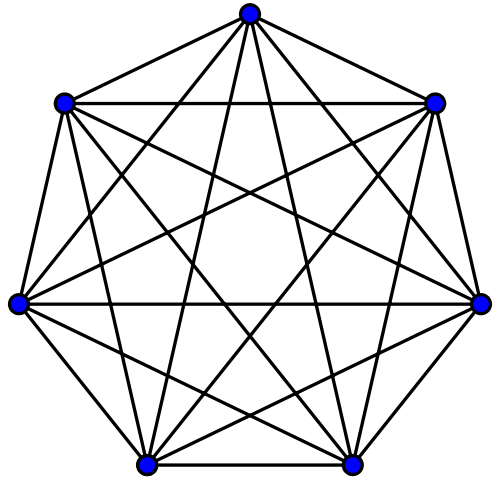
\includegraphics[width=0.55\textwidth]{network.png}
    \caption{Topologia de uma rede totalmente conectada}
    \label{fig:network}
\end{figure}
\vspace*{1em}

Não era plausível colocar equipamentos e ligar cabos em cada casa que desejasse
fazer ligações telefônicas, e a \textit{American Bell} desenvolveu o sistema de
comutação, que permitia ligações entre os telefones indiretamente, ou seja, sem
a ligação exclusiva entre os telefones. Dessa forma, uma central telefônica era
encarregada de conectar os telefones e criar o circuito da ligação.

As centrais telefônicas possuiam diversos painéis de comutação, os agrupamentos
destes chamados de \textit{trunks}, formando as primeiras redes telefônicas. As
redes eram conectadas entre centrais, cidades, estados e países, formando então
a PSTN.

\subsubsection{NAPs e roteamento de telefonia}

Os \textbf{NAPs}, sigla para \textit{network access point} ou
\textbf{ponto de acesso à rede}, são equipamentos que conectam os dispositivos
usados em uma rede interna à tipos de redes externas, como telefones locais de
um \textit{call center} à PSTN. Suas aplicações são bastante amplas, não se
limitando a essa área.

Para além da PSTN, as NAPs tambem são usadas para roteamento de chamadas e
mensagens, ou seja, direcionar o tráfego para e a partir dos terminais, os
telefones e outros dispositivos que respondem e requisitam chamadas e recebem
mensagens, tanto da rede externa com a rede externa como de telefones que se
comunicam na rede interna, a exemplo dos ramais.

Não apenas telefones se comunicam pelos NAPs, mas outros dispositivos como
porteiros eletrônicos e funções especiais de telefones híbridos, utilizando
dispositivos chamados \textbf{PABX}.

\subsubsection{Telefonia VoIP}

O \textbf{VoIP}, sigla para \textit{voice over IP} ou
\textbf{voz sobre protocolo de internet}, é um sistema de transmissão de áudio,
focado em conversação, utilizando da internet ou de outra rede de computadores
estabelecida e baseada no protocolo de internet, o protocolo IP, fazendo com
que seja um serviço bastante disponível e de baixo custo devido à ubiquidade da
internet, conectando múltiplos dispositivos como demonstrado na
figura~\ref{fig:voip}.

\vspace*{1em}
\begin{figure}[ht]
    \centering
    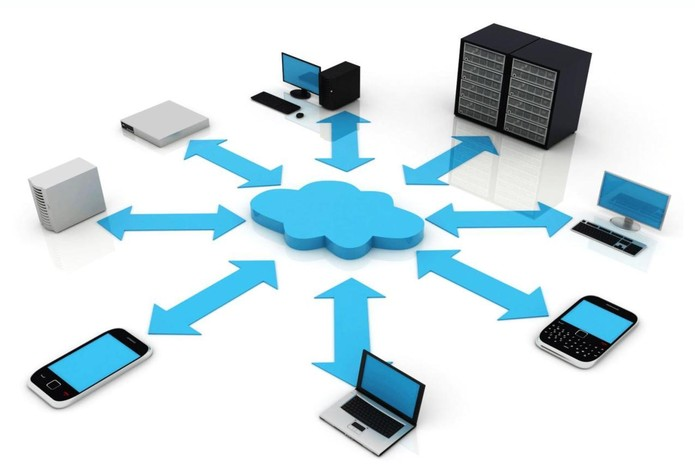
\includegraphics[width=0.75\textwidth]{voip.jpg}
    \caption{Diagrama da comunicação VoIP}
    \label{fig:voip}
\end{figure}
\vspace*{1em}

Para um usuário doméstico, o VoIP geralmente não possui custo adicional com
alguns softwares, mais conhecidamente \textbf{Skype}, da Microsoft, e uma parte
do \textbf{FaceTime}, da Apple, e não é necessário contratar um serviço
dedicado já que a rede costuma ser subutilizada e ter conexão razoável.

Já existem algumas provedoras de telefonia VoIP no Brasil, embora sofram com um
forte \textit{lobby} das grandes operadoras de telecomunicações. As empresas
provedoras de VoIP não necessitam de licença da Anatel se não fornecerem
estrutura para os clientes.

O sistema VoIP é muito mais simples e dinâmico do que a telefonia comum, uma
vez que um endereço VoIP é sempre atrelado ao mesmo dispositivo e não depende
de área e operadora. Além disso, ao usar a internet, os custos de operação do
VoIP não dependem da localização geográfica dos participantes e nem do horário
da ligação, dois fatores que alteram os preços de forma negativa na telefonia
comum.

O VoIP geralmente faz parte de sistemas com outros serviços de facilidades,
como a conversação em vídeo, as conferências de conversação, mensagens
instantâneas e compartilhamento de arquivos, e funcionam tanto em redes fixas
quanto na telefonia móvel, a exemplo do \textbf{WhatsApp} e das outras
ferramentas citadas anteriormente. Estes serviços também podem ser chamados de
\textbf{UCoIP}, sigla para \textit{unified communication over IP} ou
\textbf{comunicação unificada sobre protocol de internet}.

Para empresas, o VoIP tem diversas vantagens sobre a telefonia comum, porque é
mais fácil de fazer sua integração com outros sistemas automatizados e
computadorizados usando a mesma rede. O VoIP pode se comunicar com a PSTN por
meio de um \textit{gateway}, uma forma de NAP, que funciona como os serviços
de DNS, mapeando números indicativos dos telefones com o endereço IP do cliente
ou servidor.

\subsubsection{Protocolo SIP}

A telefonia sobre IP utiliza o protocolo \textit{SIP}
(\textbf{session initiation protocol}), um protocolo de código aberto no nível
da camada de aplicação, e que funciona no modelo ``requisição-resposta'', como
o protocol HTTP, utilizado para transferência de páginas da web. Ele funciona
de forma independente do conteúdo da transmissão, sendo também usado para
transmissão de outros tipos de mídia.

Na arquitetura do SIP, existe a estação final, chamada de agente, que pode agir
como cliente ou servidor dependendo se deseja iniciar a chamada ou se está
respondendo a uma solicitação. Um agente SIP possui um endereço parecido com um
email, na forma \textit{sip:username@domain.com}. Servidores de \textit{proxy}
podem suportar funções de encaminhamento e contabilidade de chamadas.

\subsection{Metodologia}

Na Khomp, as tarefas são divididas e distribuídas entre os desenvolvedores de
acordo com sua disposição e conhecimento. Para estagiários, estão disponíveis
algumas tarefas mais simples, como correções de bugs, mas o desenvolvedor é
livre para escolher alguma tarefa mais complexa conforme julgue ser capaz.

Após a leitura e conhecimento dos equipamentos e programas, foi sugerido pelo
coordenador da área algumas tarefas iniciais para primeiro contato com os
códigos e esquemas de organização.

\subsubsection{Protocolos e portas SIP}

O primeiro trabalho desenvolvido foi implementar a possibilidade de aceitar
qualquer tipo de transporte nos NAPs que utilizam o protocolo SIP. O SIP só faz
a comunicação de sessão e atua na camada de aplicação, portanto o
\textit{gateway} precisa usar um protocolo de transporte, que pode ser TCP,
UDP, TLS (apenas para o SIP) e SRTP (apenas para os dados), como no modelo OSI
no diagrama da figura~\ref{fig:osi}.

\vspace*{1em}
\begin{figure}[ht]
    \centering
    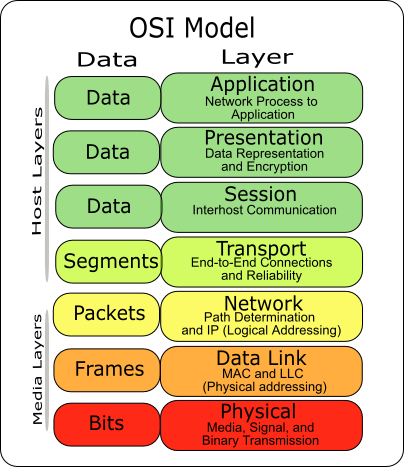
\includegraphics[width=0.45\textwidth]{osi.png}
    \caption{Diagrama das camadas do modelo OSI}
    \label{fig:osi}
\end{figure}
\vspace*{1em}

O \textit{software} da Khomp permite escolher um desses protocolos de
transporte para ser usado exclusivamente para cada protocolo de aplicação, mas
a alteração feita permitiu que o cliente possa aceitar todos os protocolos.
Como o \textit{software} já suporta todos esses protocolos, implementados no
sistema operacional, essa opção é desejada.

Além disso, quando usando TCP, a transmissão pode usar qualquer porta da rede,
que é escolhida na negociação de transporte, antes mesmo do SIP começar a ser
usado. O comportamento padrão, de usar uma porta específica, não funciona
corretamente com TCP por causa disso. Uma alteração agora força a opção de
ignorar a porta de entrada (ou seja, aceitar outras que não uma porta
predefinida) quando se usa TCP.

A primeira dessas alterações é implementada no \textit{software}, com uma
configuração gravada, e a segunda é uma alteração na interface web de controle
do \textit{gateway}.

\subsubsection{Temporização de sessões SIP}

As seções SIP precisam ser renovadas com uma certa periodicidade, uma prática
conhecida como \textit{keep-alive} e usada em outros protocolos, para garantir
que os lados de uma chamada ainda estão disponíveis. Caso um tempo definido na
negociação da seção passe e o lado atendente não envie um novo pacote, a
sessão é encerrada forçadamente.

O \textit{software} já possuía suporte para os temporizadores, mas não
utilizava. A alteração permitiu que o \textit{gateway}, que atua como
\textit{proxy}, possa atuar como mediador da sessão, negociando tempos
diferentes com os lados de uma sessão e encerrando a chamada ou mantendo-a
aberta conforme necessário.

\subsubsection{Alocadores de saída SMS}

Os \textit{gateways} da Khomp para redes GSM (redes de celular) também podem
gerenciar envio e recebimento de mensagens SMS, em um subsistema separado. Esse
sistema utilizava um alocador do tipo \textit{first-free}, que escolhe o
primeiro canal disponível em ordem para envio de SMS.

O problema dessa abordagem é que ela tende a concentrar as mensagens nos
primeiros canais, por muitas vezes sobrecarregando-os, e subutilizando os
demais, por verificar sempre à partir do primeiro canal. São necessários outros
algoritmos de alocação para balancear a alocação dos canais.

O sistema utilizava uma configuração \textit{hardcoded}, inalterável, e foi
feita uma refatoração que permite selecionar um alocador diferente a partir da
configuração ou com o \textit{software} em execução. Além do alocador já
existente, também foi desenvolvido um alocador \textit{round robin}, que é mais
conhecido por seu uso em alocadores de processos, como visto na
figura~\ref{fig:rr}.

\vspace*{1em}
\begin{figure}[ht]
    \centering
    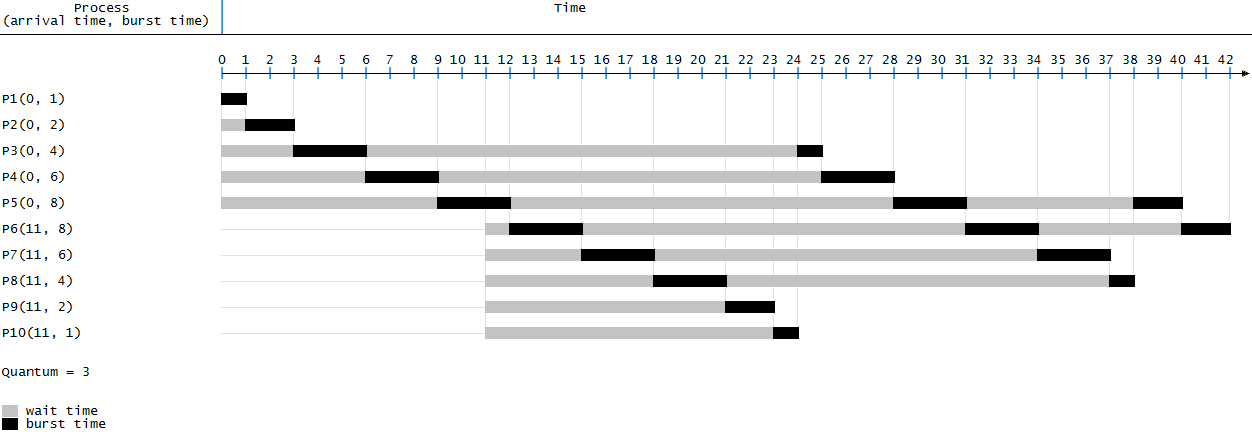
\includegraphics[width=\textwidth]{roundrobin.png}
    \caption{Alocação de processos usando \textit{round robin}}
    \label{fig:rr}
\end{figure}
\vspace*{1em}

O \textit{round robin} consiste em percorrer uma lista de recursos em ordem,
continuando a partir do último recurso disponível em vez do começo. Dessa
forma, um recurso só torna a ser novamente selecionado depois de todos os
outros serem usados ao menos uma vez. Isso não cria uma tendência em um certo
ponto dessa lista, mas espalha melhor a alocação entre todos os recursos.

Além disso, ficou como legado um \textit{framework} que simplifica bastante
futuros alocadores de serem implementados. Algoritmos específicos, por exemplo
caso o cliente desejar sempre usar o canal com o custo mais baixo ou que tenha
mais mensagens disponíveis, serão facilmente implementados.

\subsubsection{Renovação de cotas}

Ainda falando sobre alocação de canais, os canais GSM são atrelados a um chip
de uma operadora telefônica, e estas possuem franquias bastante variadas. O
\textit{software} da Khomp apenas suportava franquias com renovação mensal, mas
alguns planos mais recentes possuem renovação semanal e até mesmo diária, em
vez de renovarem num dia específico.

O \textit{software} foi alterado para permitir a seleção desses outros períodos
de franquias, com o cliente selecionando o momento em que a franquia é renovada
(hora do dia, dia da semana ou dia do mês).

\subsection{Resultados obtidos}

O \textit{software} é desenvolvido há bastante tempo, é sólido e estável, mas
sempre há potencial para melhorias. As funções adicionadas no desenvolvimento
fazem com que seja mais dinâmico em alguns pontos, e também pode prevenir
alguns bugs e inconveniências. Embora as alterações até então implementadas
sejam referentes à comportamentos de partes já existentes, em futuras tarefas
serão desenvolvidos novos sistemas.

O estágio traz conhecimento sobre uma área abordada parcialmente no curso, a de
telecomunicações, que é citada como conteúdo das disciplinas de redes e
sistemas multimídia, mas que como já mencionado não são tão aprofundadas. Dessa
forma, se faz necessário estudo e a experiência é de aprendizado constante.

\section{Conclusões}

O estágio é abrangente e permite ao estagiário trabalhar em diversos ambientes,
desde o \textit{software} em baixo nível que é utilizado diretamente no
\textit{hardware} desenolvido na própria empresa como na interface com o
usuário, bem como na integração entre esses sistemas.

O mercado em que a empresa atua precisa de profissionais de TI que tenham
experiência em engenharia de software e redes além de telecomunicações. Neste
sentido a empresa, proporciona o espaço necessário para o complemento dessa
capacitação.

A experiência de trabalhar em equipe é interessante, pois a equipe se reune com
frequência para divulgar seus resultados e é bastante integrada ao consultar
entre si as melhores soluções para os problemas. Há um bom clima que permite
que o estagiário se desenvolva e possa melhorar suas habilidades e obter
conhecimento.

%\bibliographystyle{sbc/sbc}
%\bibliography{relatorio}

\end{document}
